\lab{PageRank Algorithm}{PageRank Algorithm}
\label{lab:PageRank}
\objective{Implement the PageRank Algorithm and understand the theory behind it.}

When you enter keywords into Google's search engine, Google finds every page containing your keywords and lists the pages in order of their \emph{rank}.
The rank of a page reflects many factors, including how often the page is visited and how connected it is to other pages.
As of 2013, the PageRank algorithm is one of over 200 algorithms that Google uses to determine the rank of a website.
Named for Larry Page, cofounder of Google, this algorithm ranks pages based on how many other pages link to them.

The PageRank algorithm is also used in applications other than internet search engines.
For example, it has been used to rank graduate institutions and the impact factor of journals, and it has been used in some biological applications.

\section*{The Internet as a Graph}
The PageRank algorithm models the internet with a directed graph. 
Each webpage is a node, and there is an edge from node $i$ to node $j$ if page $i$ links to page $j$.
Let $\In(i)$ be the websites linking to page $i$ and let $\Out(i)$ be the websites that page $i$ links to. 
That is, $\In(i)$ is the set of nodes with an arrow to node $i$, and $\Out(i)$ is the set of nodes with an arrow from node $i$.
An example is illustrated in Figure \ref{fig:network1}.

\begin{figure}
\centering
\begin{tikzpicture}[node distance=1.75cm, thick ]

\node[draw=none](2)[]{2};
\node[draw=none](3)[right of=2]{3};
\node[draw=none](4)[right of=3]{4};
\node[draw=none](5)[right of=4]{5};
\node[draw=none](6)[right of=5]{6};
\node[draw=none](1)[above of=3]{1};
\node[draw=none, node distance=2.5cm](0)[right of=1]{0};
\node[draw=none](dummy)[above right of=0]{};
\node[draw=none, node distance=.5cm](7)[below 
	of=dummy]{7};

\foreach \x/\y in {3/2, 4/5, 5/6, 1/0, 3/0, 4/0, 5/0} \draw[->, 
	>=stealth'](\x)--(\y);
\draw[->, >=stealth'](6)--(0);
\draw[->, >=stealth', shorten >= .1cm](7)edge[bend left=20](0);
\draw[->, >=stealth', shorten <= .1cm](0)edge[bend left=20](7);
\draw[->, >=stealth', shorten <= .1cm](3)edge[bend right=40](6.9,-.25);
\draw[->, >=stealth', shorten <= .1cm](4)edge[bend right](6);



\end{tikzpicture}

\caption{A directed graph can describe the links between webpages. In this example, the set of web pages linking to page 0 is $\In(0)=\{1,3,4,5,6,7\}$, and page 0 links to $\Out(0)=\{7\}$.}
\label{fig:network1}
\end{figure}

The PageRank algorithm ranks pages based on how many other pages link to them.
Moreover, a link from a more important page counts more than a link from a less important page.
For example, in Figure \ref{fig:network1} we would expect node 0 to have a very high rank because every other node links to it. 
Consequently, we would expect node 7 to have a fairly high rank because node 0 links to it, even though node 0 is the only node to do so.

\section*{The PageRank Algorithm}
The PageRank algorithm assumes that a surfer chooses a starting webpage randomly.
Then, if the surfer is at page $i$, they randomly select a page from $\Out(i)$ to visit next.
This means that the surfer's chance of being on page $i$ at time $t$ is determined by where they were at time $t-1$.

Suppose the internet has $N$ webpages and let $p(i,t)$ be the likelihood that the surfer is on page $i$ at time $t$.
Then the probabilities $p(i,t)$ are given by
\begin{equation}\label{equ:pr1}
p(i,0)=\frac{1}{N} \qquad p(i,t+1) = \sum_{j \in \In(i)} \frac{p(j,t)}{\abs{\Out(j)}}.
\end{equation}

For example, in Figure \ref{fig:network1} we have $N=8$, and 
\[
p(6, t+1)=\frac{p(3,t)}{3}+\frac{p(4,t)}{3} + \frac{p(5,t)}{2}.
\]

\subsection*{Refining the Model: Pages with No Outbound Links}
A node with no outbound links is called a \emph{sink}. 
For example, node 2 in Figure \ref{fig:network1} is a sink.
According to our model, if the surfer ever visits a sink, they will stay there forever.

This is not very realistic; in this situation, a person would likely select another webpage at random and begin surfing again.
Hence, in our model we replace sinks with nodes linking to every other page. 
For example, we replace Figure \ref{fig:network1} with Figure \ref{fig:network2}.

\begin{figure}
\centering
\begin{tikzpicture}[node distance=1.75cm, >=stealth', thick]

\node[draw=none](2)[]{2};
\node[draw=none](3)[right of=2]{3};
\node[draw=none](4)[right of=3]{4};
\node[draw=none](5)[right of=4]{5};
\node[draw=none](6)[right of=5]{6};
\node[draw=none](1)[above of=3]{1};
\node[draw=none, node distance=2.5cm](0)[right of=1]{0};
\node[draw=none](dummy)[above right of=0]{};
\node[draw=none, node distance=.5cm](7)[below 
	of=dummy]{7};


\draw[->, color=black!35!](2)--(1);
\draw[->, color=black!35!, shorten >= .2cm](2)--(0);
\foreach \x/\y in {2/3, 2/4, 2/5} \draw[->, color=black!35!](\x)
	edge[bend right](\y);

\draw[->, shorten <= .1cm, color=black!35!](2)edge[bend right=50](7,-.35);
\draw[->, shorten <= .1cm](3)edge[bend right=40](6.9,-.25);
\draw[->, shorten <= .1cm](4)edge[bend right](6);
\draw[->, shorten <=.1cm, color=black!35!](2)edge[bend left=40](7);

\draw[->, shorten >= .1cm](7)edge[bend left=20](0);
\draw[->, shorten <= .1cm](0)edge[bend left=20](7);

\foreach \x/\y in {3/2, 4/5, 5/6, 1/0, 3/0, 4/0, 5/0} \draw[->, 
	>=stealth'](\x)--(\y);
\draw[-> ](6)--(0);

\end{tikzpicture}

\caption{This figure arises from Figure \ref{fig:network1} by adding a link from page 2 to every other page (the added links are grey). The new links guarantee that page 2 is no longer a sink, as required by the PageRank algorithm.}
\label{fig:network2}
\end{figure}

\subsection*{Refining the Model: Adding Boredom}
The equations in \eqref{equ:pr1} describe the surfer's habits as a Markov chain.
However, the model is more realistic if we add the assumption that the surfer sometimes gets bored and randomly picks a new starting page.
We will denote the probability that a surfer stays interested at step $t$ by a constant $d$, called the \emph{damping factor}.
Then the probability that the surfer gets bored at time $t$ is $1-d$.
Accounting for boredom, the formulas in \eqref{equ:pr1} become
\begin{equation}\label{equ:pr2}
p(i,0)=\frac{1}{N} \qquad p(i,t+1) = d\sum_{j \in \In(i)} \frac{p(j,t)}{\abs{\Out(j)}}+\frac{1-d}{N} .
\end{equation}


\subsection*{Matrix Form of the PageRank Algorithm}
We can rewrite \eqref{equ:pr2} as the matrix equation
\begin{equation}\label{equ:pr3}
\mathbf{p}(0)=\frac{1}{N}\mathbf{1} \qquad \mathbf{p}(t+1) = dK\mathbf{p}(t) + \frac{1-d}{N}\mathbf{1}
\end{equation}
where $\mathbf{p}(t)=(p(1,t), p(2,t), \ldots, p(N,t))^T$ and $\mathbf{1} = (1,\ldots, 1)^T$, and $K$ is defined by
\[K_{ij} = \begin{cases} \frac{1}{\abs{\Out(j)}} & \mbox{ if j links to i} \\
	0 & \mbox{ otherwise.} \end{cases}\]


\subsection*{Defining Page Rank}
As given by the PageRank algorithm, the \emph{rank} of page $i$ is
\[p(i) = \lim_{t\to \infty} p(i,t).\]
In other words, the page ranks are the steady state of the modified Markov chain defined in \eqref{equ:pr3}.



\section*{Implementation in Python}
A good strategy for computing $K$ comes from writing
\[
K = (D^{-1}A)^T
\]
where $A$ is the adjacency matrix of the directed graph representing the internet and $D$ is a diagonal matrix with $D_{jj}=\abs{\Out(j)}$.
Since $\Out(j)$ can be computed from the adjacency matrix, we will begin by creating $A$.

The adjacency matrix $A$ of a directed graph has $A_{ij}=1$ if there is an edge from node $i$ to node $j$, and $A_{ij}=0$ otherwise.
For example, the adjacency matrix of the graph in Figure \ref{fig:network1} is defined below.
We use a code environment to describe $A$ so you can easily use this example to debug the problems in this lab.
\begin{lstlisting}
A = np.array([[ 0,  0,  0,  0,  0,  0,  0,  1],
              [ 1,  0,  0,  0,  0,  0,  0,  0],
              [ 0,  0,  0,  0,  0,  0,  0,  0],
              [ 1,  0,  1,  0,  0,  0,  1,  0],
              [ 1,  0,  0,  0,  0,  1,  1,  0],
              [ 1,  0,  0,  0,  0,  0,  1,  0],
              [ 1,  0,  0,  0,  0,  0,  0,  0],
              [ 1,  0,  0,  0,  0,  0,  0,  0]])
\end{lstlisting}



\begin{problem}
Write the following function that creates an adjacency matrix from a file.
\begin{lstlisting}
def to_matrix( datafile, n ):
    ''' Return the nxn adjacency matrix described by datafile.
    
    INPUTS:
    datafile - A .txt file describing a directed graph. Lines 
    			describing edges should have the form 
				'<from node>\t<to node>\n'. The file may also 
				include comments.
    n		- The number of nodes in the graph described by datafile
    
    RETURN:
    Return a SciPy sparse `dok_matrix'.
    '''
\end{lstlisting}
Hints:
\begin{enumerate}
\item The file \texttt{data.txt} included with this lab describes the matrix in Figure \ref{fig:network1}. 
You may use it to test your function.

\item You can open a file in Python using the \li{with} syntax. 
Then, you can iterate through the lines using a \li{for} loop.
Here is an example.
\begin{lstlisting}
# Open `data.txt' for read-only
with open('./data.txt', 'r') as myfile:
    for line in myfile:
        print line
\end{lstlisting}

\item Here is an example of how to process a line of the form in \li{datafile}.
\begin{lstlisting}
>>> line = '0\t4\n'
# strip() removes trailing whitespace from a line.
# split() returns a list of the space-separated pieces of the line.
>>> line.strip().split()
['0', '4']
\end{lstlisting}

\item Rather than testing for lines of \texttt{data.txt} that contain comments, put all your string operations in a \li{try} block with an \li{except} block following.
\end{enumerate}
\end{problem}

The next step is to compute $K$. 
The matrix $D$ is easily obtained from $A$ (how?). 
Then, we can use $D$ to identify sinks.
Modify $A$ so that rows corresponding to sinks have all ones instead of all zeros.
For Figure \ref{fig:network2}, the modified adjacency matrix is defined below.
\begin{lstlisting}
Am = np.array([[ 0,  0,  0,  0,  0,  0,  0,  1],
               [ 1,  0,  0,  0,  0,  0,  0,  0],
               [ 1,  1,  1,  1,  1,  1,  1,  1],
               [ 1,  0,  1,  0,  0,  0,  1,  0],
               [ 1,  0,  0,  0,  0,  1,  1,  0],
               [ 1,  0,  0,  0,  0,  0,  1,  0],
               [ 1,  0,  0,  0,  0,  0,  0,  0],
               [ 1,  0,  0,  0,  0,  0,  0,  0]])
\end{lstlisting}

Finally we compute $K$.
It is a \emph{very} bad idea to invert $D$ and perform the matrix multiplication $D^{-1}A$.
Rather, store the diagonal entries of $D$ in a vector and use array broadcasting to divide $A$ by $D$.
For Figures \ref{fig:network1} and \ref{fig:network2}, the matrix $K$ is as follows.

\begin{lstlisting}
K = np.array([[ 0   ,  1   ,  1./8,  1./3,  1./3,  1./2,  1   ,  1   ],
              [ 0   ,  0   ,  1./8,  0   ,  0   ,  0   ,  0   ,  0   ],
              [ 0   ,  0   ,  1./8,  1./3,  0   ,  0   ,  0   ,  0   ],
              [ 0   ,  0   ,  1./8,  0   ,  0   ,  0   ,  0   ,  0   ],
              [ 0   ,  0   ,  1./8,  0   ,  0   ,  0   ,  0   ,  0   ],
              [ 0   ,  0   ,  1./8,  0   ,  1./3,  0   ,  0   ,  0   ],
              [ 0   ,  0   ,  1./8,  1./3,  1./3,  1./2,  0   ,  0   ],
              [ 1   ,  0   ,  1./8,  0   ,  0   ,  0   ,  0   ,  0   ]])
\end{lstlisting}
\begin{problem}
Write a function that computes the K matrix given an adjacency matrix.
\begin{enumerate}
\item Compute the diagonal matrix $D$.
\item Compute the modified adjacency matrix where the rows corresponding to sinks all have ones instead of zeros.
\item Compute $K$ using array broadcasting.
\end{enumerate}
\end{problem}


\subsection*{Solving for the Page Ranks}
There are several ways to solve for $\lim_{t \to \infty} \mathbf{p}(t)$.
\subsubsection*{Algebraic Method}
One possibility is to assume the modified Markov chain has a steady state $\mathbf{p}$ and solve for it algebraically:
\begin{equation}\label{equ:matrix_solve}
(I-dK)\mathbf{p} = \frac{1-d}{N} \mathbf{1}.
\end{equation}

We can implement this algorithm in SciPy to solve for the page ranks of the network in Figure \ref{fig:network2}.
\begin{lstlisting}
>>> from scipy import linalg as la
>>> I = np.eye(8)
>>> d = .85
>>> la.solve(I-d*K, ((1-d)/8)*np.ones(8))
array([ 0.43869288,  0.02171029,  0.02786154,  0.02171029,  0.02171029,
        0.02786154,  0.04585394,  0.39459924])
\end{lstlisting}
As expected, node 0 has the highest rank, approximately equal to .43. 
Node 7 has a much higher rank than node 6, even though $\In(7)=1$ and $\In(6)=3$. 
This is because node 7's single in-edge comes from a node that has a very high rank (node 0).

\subsubsection*{Iterative Method}
Solving the system in \eqref{equ:matrix_solve} is feasible for our small working example, but this is not an efficient strategy for very large systems.

One option for large systems is to iterate the equation for $\mathbf{p}(t)$ until $\norm{\mathbf{p}(t)-\mathbf{p}(t-1)}$ is sufficiently small.


\begin{problem}
\label{prob:pagerank_dense_iter}
Implement the function below, using the iterative method to find the steady state of the PageRank algorithm.
\begin{lstlisting}
def iter_solve( data, datasize, N=None, d=.85, tol=1E-5):
    '''
    Return the page ranks of the network described by `data`.
    
    INPUTS:
    data - A NumPy array representing the adjacency matrix of a directed 
            graph
    datasize - An integer representing the size of the 'data' array.
    N     - Restrict the computation to the first `N` nodes of the graph. 
            Defaults to N=None; in this case, the entire matrix is used.
    d     - The damping factor, a float between 0 and 1. 
            Defaults to .85.
    tol  - Stop iterating when the change in approximations to the 
            solution is less than `tol'. Defaults to 1E-5.
    
    OUTPUTS:
    Iterate through the PageRank algorithm until the error is less than 
    `tol'. Return the approximation to the steady state.
    '''
\end{lstlisting}
Hints:
\begin{enumerate}
\item At each step, test your function against the example in this lab.
\item Don't forget to eliminate sinks. 
It is possible (but not necessary) to do this in a single line.
\item When \li{N} is not \li{None}, you want to work with only the upper $N \times N$ portion of the array \li{data}.
\end{enumerate}
\end{problem}

\subsubsection*{Eigenvalue Method}
Another way to solve this problem is to make it into an eigenvalue problem. 
Let $E$ be an $N \times N$ matrix of ones; then $E\mathbf{p}(t) = \mathbf{1}$. 
Hence, the matrix equation \eqref{equ:pr3} for $\mathbf{p}(t+1)$ becomes
\[\mathbf{p}(t+1) = \Big(dK + \frac{1-d}{N}E\Big)\mathbf{p}(t).\]
If we write $B = dK + \frac{1-d}{N}E$, this simplifies to $\mathbf{p}(t+1) = B\mathbf{p}(t).$
Thus, the steady state $\mathbf{p}(t)$ is an eigenvector of $B$ corresponding to the eigenvalue 1.

The columns of $B$ sum to 1, and the entries of $B$ are strictly positive (because the entries of $E$ are all positive).
With these hypotheses, the Perron-Frobenius theorem says that 1 is the unique eigenvalue of B of largest magnitude, and the corresponding eigenvector is unique.
In this case, the ``iterative method'' described above is just the power method for finding the eigenvector corresponding to a dominant eigenvalue, introduced in Lab \ref{lab:EigSolve}.

We can also attempt to compute $\mathbf{p}$ using eigenvalue solvers in SciPy.

%TODO: the output from scipy.linalg.eig is not very accurate, even for the small example in this lab.
\begin{problem}
Implement the function below, using the eigenvalue method to find the steady state of the PageRank algorithm.
\begin{lstlisting}
def eig_solve( data, datasize, N=None, d=.85):
    '''
    Return the page ranks of the network described by `data`.
    
    INPUTS:
    data - A NumPy array representing the adjacency matrix of a directed 
            graph
    datasize - An integer representing the size of the 'data' array.
    N     - Restrict the computation to the first `N` nodes of the graph. 
            Defaults to N=None; in this case, the entire matrix is used.
    d     - The damping factor, a float between 0 and 1. 
            Defaults to .85.
    
    OUTPUTS:
    Use the eigenvalue solver in \li{scipy.linalg} to calculate the steady 
    state of the PageRank algorithm.
    '''
\end{lstlisting}
Hint: Review the techniques from the Markov chain section of Lab \ref{lab:EigSolve}.
\end{problem}


\section*{SNAP Datasets}
The SNAP graph library, located at \url{http://snap.stanford.edu/data/index.html}, provides a variety of medium sized data sets for public use.
The \li{matplotlib.pyplot.spy} command on the adjacency matrix from a SNAP data set yielded the plot shown in Figure \ref{fig:WebSparse}

\begin{figure}
\centering
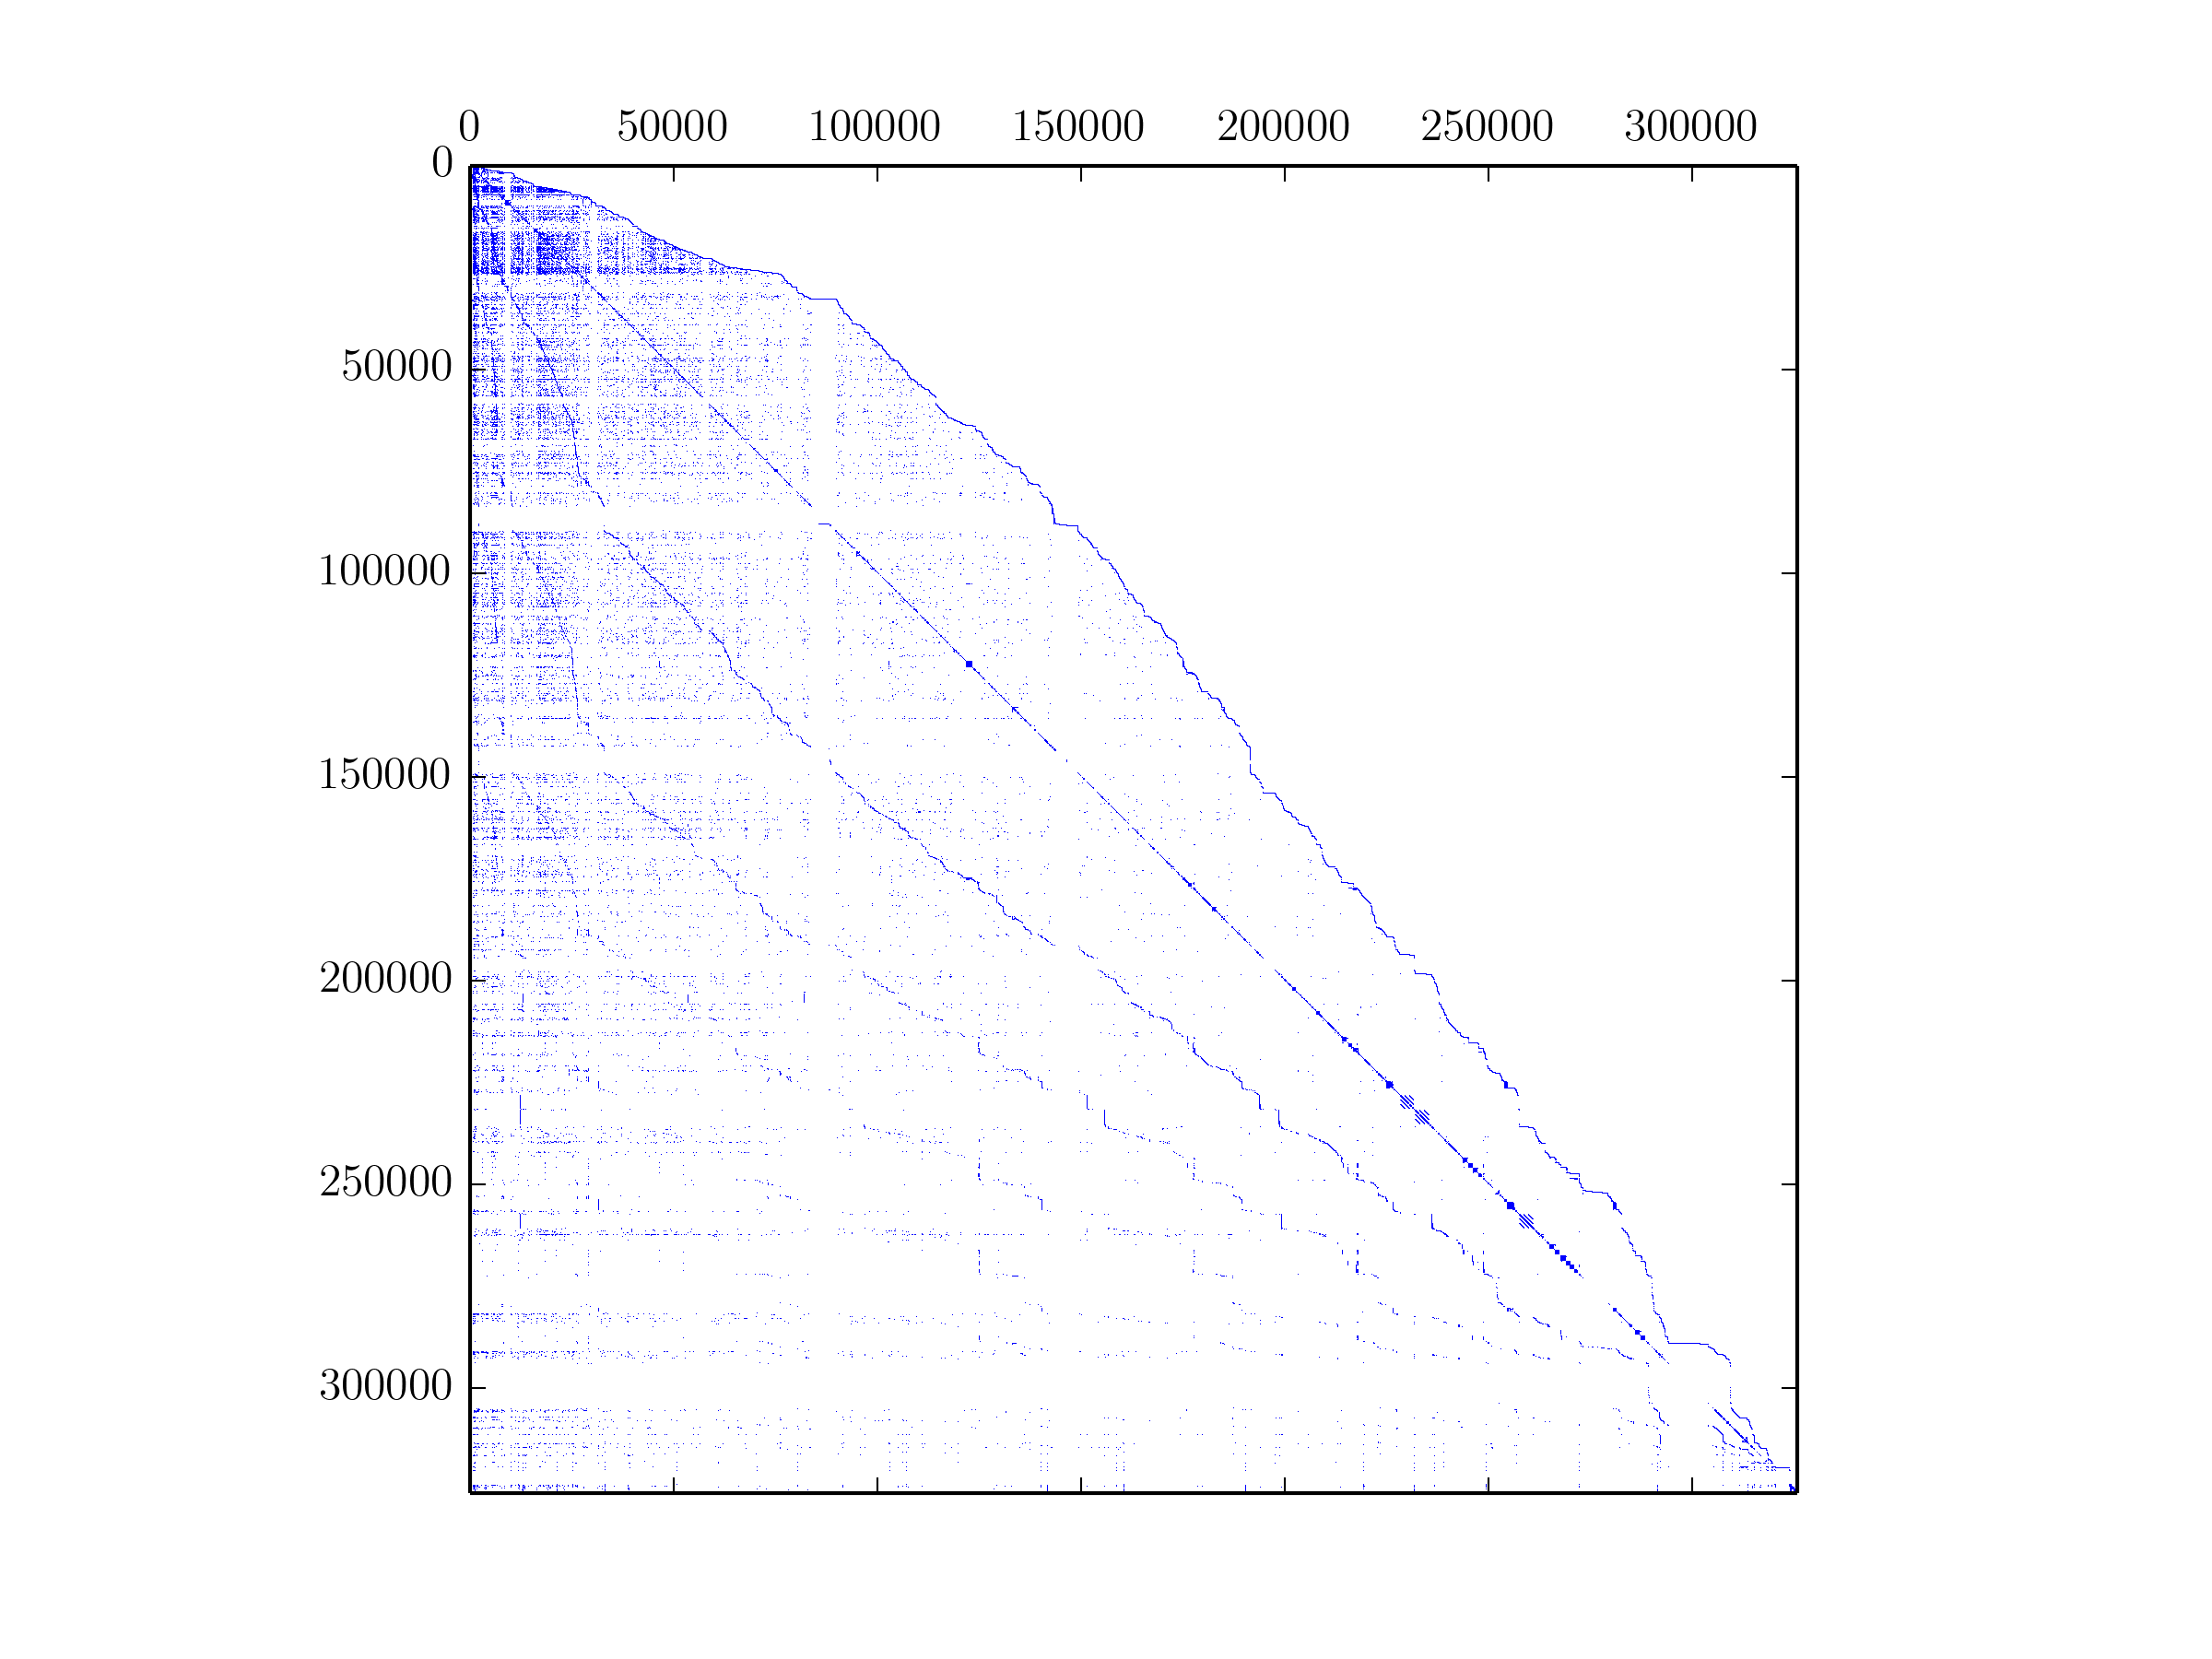
\includegraphics[width=\textwidth]{sparse_web.png}
\caption{Output of the \li{spy} command on the adjacency matrix corresponding to the websites supported by Notre Dame University in 1999.
Data was taken from the SNAP datasets.}
\label{fig:WebSparse}
\end{figure}

\begin{problem}
Try running the functions you wrote in this lab on a data set downloaded from SNAP.
\begin{enumerate}
\item Begin by running your methods on the first 100 nodes of the data set.
\item Modify your solution to Problem \ref{prob:pagerank_dense_iter} so that it uses only sparse matrices. 
With this modification, you should be able to run the function on more nodes.
Hint: Convert the adjacency matrix to a \li{csc_matrix} or a \li{csr_matrix} to perform the computations.
\end{enumerate}
\end{problem}
